\chapter{Literature Review} \label{chap:litreview} Ozone (O$_3$) formation and detection have been an interest in academics for over a century. The discovery of O$_3$ by Dr. Gordon Dobson in the early 1920s resulted in the first in-situ measurement of total column O$_3$ (TCO$_3$) by comparing UV absorption to the intensity of various wavelengths at the same time and place \parencite{dobson_measurements_1923}. The discovery of the stratospheric O$_3$ layer, development of the Dobson Spectrophotometer, and establishment of the Dobson Unit (DU) later enabled researchers to detect substantial depletion of Arctic stratospheric O$_3$, most notably the 1985 finding by \parencite{farman_large_1985}. They found the Arctic contained higher levels of inorganic chlorine (commonly denoted Cl$_n$, e.g, HCl and ClONO$_3$), which, under temperatures below ~196 \textpm 4 Kelvin (K), undergo heterogeneous activation with cloud particles. The main observation to note from their work is the conversion into reactive radicals (Cl, ClO) which catalyzed O$_3$ destruction \parencite{webster_chlorine_1993}. 

When chlorine enters this active state, catalytic O$_3$-destroying cycles will continue until the initial activated reservoirs are depleted. While O$_3$ depletion does not directly drive sea-level rise, Arctic O$_3$ loss indicates polar stratospheric cooling, which can be linked to broader climate feedback mechanisms such as the ice-albedo effect and greenhouse warming. These processes have been associated with ice melt and sea-level rise (\cite{girach_influences_2023}; \cite{minghu_ding_year-round_2020}, \cite{nadzir_spatial-temporal_2018}). O$_3$ primarily absorbs UV radiation, playing a complex roles in atmospheric chemistry by modulating the concentrations of other trace gases, such as reactive chlorine and nitrogen species, thereby acting as a catalytic agent within stratospheric cycles (\cite{farman_large_1985}; \cite{hansen_scientific_2007}; \cite{webster_chlorine_1993}; \cite{he_sensitivity_1999}).

This literature review aims to leverage a wide range of resources, including professional CUB guidance, coursework, and Big Data sources, to enhance understanding of overall surface O$_3$ formation and interactions. Despite its simplicity, characterized by three oxygen molecules, the subject presents numerous complexities with both short- and long-term trends occurring at various resolutions. Given the vast potential of computer science, this project adheres to two informal principles from the fields of computer science and military doctrine: Keep It Stupid Simple (K.I.S.S.) and Proper Planning and Preparation Prevents Piss Poor Performance (the 7P’s). Streamlined access to the data enables the utilization of a multitude of resources for project implementation across various fields. A thorough yet concise analysis of contemporary O$_3$ reaction-based models from diverse disciplines will be conducted to develop a deep understanding of surface O$_3$ reactions, independent of their occurrence. 

Literature was also gathered from colleagues and coursework completed during the writing of this thesis. The literature database utilized in this thesis provides a general background on the formation of O$_3$, supporting the development of surface O$_3$ models in PHOTUC. The models employed are expected to be consistent across most cases of complex adaptive systems (CAS). These systems typically exhibit numerous similar predictive features without an identifiable unifying principle. Consequently, significant multicollinearity is anticipated among key features for O$_3$ (\cite{alvarez-mendoza_spatial_2019}). This section aims to enhance the understanding of where surface O$_3$ reactions primarily occur, considering various physical, chemical, and biological trends. Additionally, it examines how these reactions have been incorporated into contemporary models for further integration into the RK model for improvement.
%%%%%%%%%%%%%%%%%%%%%%%%%%%%%%%%%%%%%%%%%%%%%%%%%%%%%%%%%%%%%%%%%%%%%%%%%%%%%%%%%%%%%%%%%%%%%%%%%%%%%%%%%%%%%%%%%%%%
\section{Search Methods And Literature Database Creation} \label{litreview:searchmeth} The synthesized literature employed the extensive academic resources of the University of Colorado, Boulder (CUB) to conduct a comprehensive investigation into O$_3$ mechanisms and processes associated with air pollutants. With access to a substantial body of academic literature through the CUB library, EBSCOhost, and Web of Science, various documents were selected based on keywords identified during the literature review conducted throughout the coursework. 

\begin{table}[h]
    \centering
        \begin{tabular}{|c|cccc|}
            \hline
             Topic & Category & Search Terms & EBSCO & WoS \\
            \hline
             1 & O$_3$ & surface ozone, ground ozone, O3, ozone & 112,673 & 177,569 \\
             2 & Models & boosting, machine learn, deep learn & 5,140 & 8,833 \\
             3 & Ecology & public health, pollution, chemistry & 49,081 & 68,666 \\
             4 & Human & mortality, injur*, illness*, hospital* & 8,716 & 16,200 \\
             5 & Risk & dispropo*, vulner*, risk*, burden* & 21,125 & 48,387 \\
             6 & Prediction & predict*, air qual*, air chem*, model & 51,508 & 90,932 \\
             7 & Transport & transport*, trajector*, circulat*, advection* & 17,520 & 31,633 \\
            \hline
        \end{tabular}
    \caption{Categories and Examples of Search Terms}
    \label{tab:literature-count}
\end{table}
Individual counts from each search are presented in Table \ref{tab:literature-count}. Citations gathered from these searches were imported into Python and Zotero for proper formatting and de-duplication. Many works utilized throughout this thesis, including the introduction, were sourced through this process, while others were obtained from informational meetings and coursework. A Python script accessed the API of each database using the categorization of key terms in Table \ref{tab:literature-count}. 

Certain works mentioned (e.g., \cite{dobson_measurements_1923}; \cite{farman_large_1985}; \cite{he_sensitivity_1999}) and others published before 2000 (e.g., \cite{davies_episodes_1994}; \cite{goodchild_geographical_1992}) were retained for a few reasons. Among these and other studies (e.g., \cite{farkas_surface_1979}; \cite{padro_dry_1994}; \cite{massman_review_1998}), O$_3$ chemistry and transport mechanisms have been extensively explored within the metaphorical academic cog for decades. These works also emphasize methodologies employed in numerous studies over the past decade, which are further analyzed in this chapter. The final grouping of key terms and the overarching subject of each chapter can be found in \ref{tab:thesislitcount}. \begin{table}[h!]
    \centering
    \begin{tabular}{|c|l|r|r|}
        \hline
        \textbf{Chapter} & \textbf{Set Combination} & \textbf{EBSCO} & \textbf{WoS} \\ \hline
        I   & All sets            & 29     & 196     \\ \hline
        II  & T1, T2, T6, T7      & 436    & 964     \\ \hline
        III & T1, T2, T6          & 2,365  & 4,750   \\ \hline
        VI  & T1, T3, T4, T5, T7  & 350    & 1,238   \\ \hline
        \multicolumn{3}{|c|}{Thesis Count} & 246     \\ \hline
    \end{tabular}
    \caption{Total Counts of Literature Sources}
    \label{tab:thesislitcount}
\end{table} The combinations of terms following Topic 1 (T1) in Table \ref{tab:thesislitcount} were employed to construct patterns within the abstracts and titles of the literature, facilitating the categorization of the collected material. All gathered literature was reviewed using the associated DOI with CUB credentials. For this thesis, over 1,000 unique documents related to O$_3$ were identified across both databases. Various disciplines were captured, including Environmental Sciences, Ecology, Meteorology, Atmospheric Sciences, and Public Health. Each of these fields is interested in surface O$_3$ reactions and has employed relevant techniques beneficial to this thesis (e.g., \cite{abdullah_development_2019}; \cite{ghozikali_effect_2015}; \cite{he_effects_2024}; \cite{turner_long-term_2016}; \cite{xiao_lu_exploring_2019}). 

Upon reviewing the database, this thesis identified that many sources employed various numerical models and chemical transport models (CTM) to simulate, forecast, or analyze O$_3$ behavior through sensitivity analyses (e.g., \cite{kleinert_intellio3-ts_2020}; \cite{emmons_description_2010}; \cite{ma_sensitivity_2021}). Figure \ref{fig:worldcloud} illustrates that frequently used terms, such as "ozone," "concentration," "surface," "pollutant," "model," "data," and "study," are prominent based on the titles, abstracts, and keywords of each source in the literature. \begin{figure}[h!]
    \centering
    
\includegraphics[width=0.75\linewidth]{ThesisFilePkg//figs/wordcloud_latex_subscripts.png}
    \caption{Word Cloud for Abstracts in Literature Search}
    \label{fig:worldcloud}
\end{figure} The sorting methods indicate that much of the literature effectively focuses on quantifying and analyzing O$_3$ as a pollutant. Furthermore, terms such as "simulation," "analysis," "based," "method," "measurement," and "trend" highlight the reliance on data-driven models, as well as statistical or simulation-based techniques for reporting O$_3$ trends. Locational terms like "China," "city," "urban," "station," "area," and "United States" indicate focal areas and study sites—especially in East Asia and urban environments. The similarities in utilized terminology were used to categorize the literature into three main categories, as shown in Figure \ref{fig:venn}.

\begin{figure}[h!]
    \centering
    
\includegraphics{ThesisFilePkg/figs/VennDiagram.png}
    \caption{Total Counts of Literature Sources}
    \label{fig:venn}
\end{figure} Each category was based on transport, modeling, and the impact of O$_3$ literature gathered through a mass search. Modeling comprised papers that primarily mentioned keywords from topics 1 and 2. Transport relates to topics 1 and 7. The remaining categories were associated with health, featuring overlapping terms such as "effect," "impact," "change," "quality," "emission," "exposure," and "climate." These terms reflect O$_3$’s relevance to air quality, human health, and climate interactions. Further analysis of the literature indicated a recent increase in interest concerning O$_3$ production at the surface. A majority of these factors are noted in the area of interest (AOI) within this study.
%%%%%%%%%%%%%%%%%%%%%%%%%%%%%%%%%%%%%%%%%%%%%%%%%%%%%%%%%%%%%%%%%%%%%%%%%%%%%%%%%%%%%%%%%%%%%%%%%%%%%%%%%%%%%%%%%%%%
\section{Surface O$_3$ Formation and Transport} \label{litreview:sofat} The word cloud in Figure \ref{fig:worldcloud} highlights common factors such as "VOCs," "precursor," and "temperature," which emphasize frequently referenced O$_3$ precursors and meteorological conditions. Words like "year", "period", "daily", "summer", "trend", and "long term" show the potential temporal resolution of O$_3$ studies. Interpretation of the literature shows the rate of O$_3$ reactions exhibit seasonal and anthropogenic patterns at extremely close distances. Unlike most pollutants, surface O$_3$ tends to cyclically increase at distal locations from non-maintained and overly-maintained spaces (\cite{choi_summertime_2012}; \cite{damico_cyclic_2024}; \cite{guan_summer_2023}; \cite{kim_modeling_2016}; \cite{oltmans_seasonal_1992}). Figure \ref{fig:literatureot} illustrates the growing interest in this type of research since the establishment of the EPA in 1970. \begin{figure}[h!]
    \centering
    
\includegraphics[width=0.8\linewidth]{ThesisFilePkg//figs/pubot.png}
    \caption{Counts of Literature Over Time}
    \label{fig:literatureot}
\end{figure} Recent studies have shown that surface O$_3$ formation follows seasonal patterns of high and low concentrations, steadily increasing in urban areas over time due to interactions with solar radiation (UV) and VOCs (\cite{alves_first_2024}; \cite{chen_characteristics_2022}; \cite{perera_nox-voc-o3_2019}). The constituents and drivers of O$_3$ might have a heavy effect on urban layouts where geophysical systems force higher temperatures to heavily populated areas. When the separation between urban density and available green space is substantial, surface O$_3$ reactions tend to occur in areas with high biological activity or in regions prone to natural hazards associated with heat and aerosol movement, such as storms, heat waves, and volcanic eruptions (\cite{brown-steiner_asian_2011}; \cite{badia_modelling_2023}; \cite{han_modeling_2018}; \cite{place_sensitivity_2023}). Although the latter may not be found in most areas in the USNA, communities downwind of golf courses, urban parks, and similar anthropogenic constructions may experience the brunt of O$_3$ concentrations due to these transport mechanisms (\cite{al-qassimi_ozone_2020}; \cite{kong_unraveling_2023}; \cite{monks_tropospheric_2015}). 
%%%%%%%%%%%%%%%%%%%%%%%%%%%%%%%%%%%%%%%%%%%%%%%%%%%%%%%%%%
\subsection{Complexities of Urban Surface O$_3$} \label{subs:sofat1} The ideal distance for the proper representation of patterns regarding surface O$_3$ have yet to be formally established \cite{abdullah_development_2019}; \cite{tong_characteristics_2017}; \cite{wang_does_2023}) due to the interaction of O$_3$ molecules in urban environments. Unlike most pollutants, surface O$_3$ concentrations tend to cyclically increase with interactions within anthropogenic spaces (\cite{choi_summertime_2012}; \cite{damico_cyclic_2024}; \cite{guan_summer_2023}; \cite{kim_modeling_2016}; \cite{oltmans_seasonal_1992}). Similarities across study areas have revealed that surface O$_3$ exhibits seasonal high and low concentrations during the summer and winter, respectively, while steadily increasing over time in urban areas due to interactions with solar radiation and VOCs. This pattern is particularly noted when winter may not be as cold, influenced by the overall geography of the AOI (\cite{alves_first_2024}; \cite{guan_summer_2023}; \cite{perera_nox-voc-o3_2019}). 

In Chapter \ref{chap:introchap}, it was noted that the formation of surface O$_3$ is induced by stable tropospheric O$_3$ cycles when the area experiences consistently high temperatures and the presence of specific constituents, as observed in the AOI of this thesis. Large populations can significantly contribute to O$_3$ formations and are particularly vulnerable to complex variations due to substantial disparities in access to green spaces and industrialized zones (\cite{pan_vertical_2024}; \cite{cai_oxidative_2022}; \cite{meo_effect_2021}). In addition, at low temperatures and combined with severely polluted, low photolysis days will typically denote lower O$_3$ concentrations \cite{he_sensitivity_1999}; \cite{jimenez_ozone_2004}; \cite{manzini_detection_2024}). The locations of these spaces do not adhere to general, non-spatial patterns, and pollutants exhibiting spatial non-heterogeneity at small distances must be properly correlated with their sources. 
%%%%%%%%%%%%%%%%%%%%%%%%%%%%%%%%%%%%%%%%%%%%%%%%%%%%%%%%%%
\subsection{Modern Numerical Models and Overcoming Adversity} \label{subs:sofat2} This nature, applying a model for individual participants over a designated space and time is arduous work. This thesis presents a high spatial resolution model of surface O$_3$ values, utilizing similar high-resolution techniques across three counties in Arizona. While Pima, Pinal, and Maricopa counties were chosen due to their population densities; this project results in reproducible functions for all areas with the appropriate materials due to innovations made to GIScience \cite{goodchild_mapping_2018}. Atmospheric conditions, constituents, model types, and depictions of surface O$_3$ here build an basis for the final tuning metrics used to represent outputs.

Trends and transportation mechanisms should be represented in the final display over the main urban areas in the Area of Interest (AOI), Phoenix and Tucson (PHOTUC), reflecting the information discussed in this section. The recent revolution in Big Data and complex modeling techniques has enabled approaches that extend beyond traditional linear frameworks. These innovative methods incorporate transport, anthropogenic, and thermodynamical mechanisms into feature bases for urban locations (\cite{chiacchiaretta_inland_2024}; \cite{gagliardi_machine_2020}; \cite{yu_errors_2018}). Modeling techniques for training, validation, prediction and implementation with the residual kriging method are noted and discussed further in the methods section. Studies such as (\cite{yu_errors_2018}; \cite{zhou_coupling_2018}) utilize CTM based methods to combine atmospheric dynamics and satellite imagery (\cite{lin_intercomparison_2024}). 

Some researchers like (\cite{rovira_air_2020}) utilized statistical methods called DALYs for public health to assign O$_3$ exposures to individuals within a distance to nearest monitor methodology. These assessments must be conducted for each study or cohort, considering each participant or location. A study spanning numerous states, spans exponentially more counties and subsequent data points necessary for conclusive analysis (e.g., \cite{chen_association_2023}; \cite{gogna_cohort_2024}; \cite{rovira_air_2020}).  Additionally, careful consideration of co-funding factors, such as heat in urban ecologies and wildfires, is essential for the proper modeling of  (\cite{lee_wildfire_2024}; \cite{reid_role_2012}; \cite{watson_machine_2019}).
%%%%%%%%%%%%%%%%%%%%%%%%%%%%%%%%%%%%%%%%%%%%%%%%%%%%%%%%%%%%%%%%%%%%%%%%%%%%%%%%%%%%%%%%%%%%%%%%%%%%%%%%%%%%%%%%%%%%
\section{Chemical Transport Models} \label{litreview:ctms} CTMs and ML ensembles represent distinct modeling paradigms; CTMs are process-based and mechanistic, while ML ensembles are data-driven. Recent studies demonstrate they can be effectively combined to improve surface O$_3$ forecasting accuracy at coarse resolutions (\cite{sun_improvement_2021}; \cite{yu_errors_2018}; \cite{cheng_improvement_2022}) which can later be aggregated to a finer resolution. Typically, CTMs and ML ensembles sit at opposite ends of the modeling spectrum, but they can complement one another when studying pollutants such as surface O$_3$. ML ensembles don’t deal with spatial data; they’re combined with CTMs which are a mechanistic, three-dimensional (3D) Eulerian framework accounting for some spatial variation through linear associations over a large trend predicted by the ensemble (\cite{balamurugan_tropospheric_2021}; \cite{travis_systematic_2019}; \cite{kang_estimation_2021}). Most CTMs were found to have approximately 8 to 13 ppb with a 5 ppb RMSE associated with their predictions (\cite{kalbande_machine_2023}; \cite{travis_systematic_2019}; \cite{wang_novel_2020}) likely attributable to the modifiable unit area problem (MAUP) encountered when resampling outputs to achieve the desired higher resolution \cite{manley2014}. 

CTMs separate emissions and transport mechanisms to model the relationships between surface measurements and satellite detections. They typically incorporate valuable spatial information into the overall error of the associated model, rather than accounting for geospatial uncertainty (\cite{konovalov_inverse_2006}; \cite{lin_model_2012}; \cite{minarro_study_2011}; \cite{rojas_uncertainty_2016}). Furthermore, CTMs are both computationally and temporally costly. Most models require extensive access to Big Data systems and expensive technology for accurate depictions of surface trends (\cite{brown_running_1995}; \cite{keller_machine_2017}). CTMs that incorporate ML and AI methods for transport can be further enhanced by effectively integrating geospatial uncertainty from monitored data through residual kriging. This approach improves the reliability and value of these costly systems in light of increased accessibility to monitoring data. Their transport representations depend on continuity equations such as advection, convection, emissions, and detailed gas and/or aqueous phase interactions, along with other atmospheric equations and chemistry (\cite{petetin_model_2021}).

Proper incorporation of numerical models is essential, as uncertainties in general aerosol models are significantly greater (\cite{lin_modeling_2012}; \cite{minarro_study_2011}; \cite{rojas_uncertainty_2016}. CTMs typically utilize meteorological data derived from remote sensing and employ selected chemical mechanisms to simulate concentrations across scales from global to rural, achieving higher-than-average spatial and temporal resolutions. These physically coherent fields are suitable for investigating chemical lifetimes, transport, and stratosphere–troposphere cycles of certain chemicals; however, extremely reactive molecules such as O$_3$ often yield the highest errors. The general laws of physics applied within CTMs are extracted and utilized in feature creation, which is discussed later in Chapter \ref{methods}.
%%%%%%%%%%%%%%%%%%%%%%%%%%%%%%%%%%%%%%%%%%%%%%%%%%%%%%%%%%%%%%%%%%%%%%%%%%%%%%%%%%%%%%%%%%%%%%%%%%%%%%%%%%%%%%%%%%%%
\section{Statistical Regression} \label{litreview:sm} CTMs have used linear regression to model associations with anthropogenic sources. Linear regression is a well-established statistical method for regression and prediction (\cite{sun_prediction_2015}; \cite{wang_combining_2016}). Its simplicity, interpretability, and efficiency render it a valuable tool for geographic predictions, particularly in binary classification scenarios, such as land cover changes, habitat presence, or the classification of environmental hazards (\cite{starbuck_linear_2023}). Linear regression is incredibly straightforward, typically denoted by the notation:
\[
f(x) = m(x) + b + \varepsilon
\]
where $m(x)$ is an indirect rise-over-run correlation between the independent variable and a specific feature, $b$ represents the y-intercept, and $\varepsilon$ indicates the residual error that each point x deviates from the mean trend. Extending this equation to multiple covariates leads to multi-linear regression:
\[
y(x) = \beta_0 + \beta_1 x_1 + \beta_2 x_2 + \cdots + \beta_i x_i + \varepsilon
\]
where each $\beta_i$ represents a weighted value attributed to $y(x)$ \cite{starbuck_linear_2023}. There are minimal interpretations to consider, and linear methods typically require little tuning unless additional weighting techniques are employed. However, surface O$_3$ entails greater complexity. CTMs offer these complex relationships attributing to linear correlations for effective modeling strategies (\cite{napi_different_2023}). Although linear regression is often applied alongside Principal Component Analysis (PCA) and Artificial Neural Networks (ANN) (\cite{moustris_application_2012}; \cite{sun_prediction_2015}), O$_3$ trends cannot be modeled at high resolutions with something unable to consider complex systems. This thesis seeks to utilize linear scopes for feature analysis, but it has been found that non-linear approaches have better results over the past decade( \cite{cavaliere_development_2023}; \cite{li_development_2024}). Machine Learning (ML) and Artificial Intelligence (AI) methods operate with increased complexity, learning weights by aggregating samples into statistically related bins—a process commonly referred to as boosting.
%%%%%%%%%%%%%%%%%%%%%%%%%%%%%%%%%%%%%%%%%%%%%%%%%%%%%%%%%%%%%%%%%%%%%%%%%%%%%%%%%%%%%%%%%%%%%%%%%%%%%%%%%%%%%%%%%%%%
\section{Machine Learning} \label{litreview:ml} Modern CTM models employ a combination of statistical trends and weighted boosting methods to learn from the meteorological tendencies present in the dataset through Machine Learning (ML). While CTMs provide accurate depictions of atmospheric physics and can utilize ML methods, they do not inherently learn from data. Rather, they are features for use in an ML model, and carry their own spatial uncertainties requiring corrections from the researcher (\cite{yu_errors_2018}; \cite{travis_systematic_2019};\cite{xiong_improved_2024}). CTMs come at a high computational cost, often resulting in hundreds to thousands of CPU-hours for resolutions of 500 m to 1 km. They are also dependent on emission inventories and parameterizations that carry additional uncertainties (\cite{chen_comparison_2021}; \cite{gilliland_dynamic_2008}; \cite{han_modeling_2018}). Utilizing these to represent 100 m-300 m of space is unsuitable due to the uncertainty in model error at these resolutions. CTMs are grounded in standard representations of tropospheric–stratospheric chemistry, including models such as (MOZART-TS1; \cite{meiyun_lin_us_2016}), the Community Earth System Model (CESM; \cite{kan_yi_response_2016}), and the multi-model reanalysis of Surface O$_3$ (MUSICA; \cite{lin_intercomparison_2024}).

Most CTMs are tree-based algorithms, as they implement complex trends to create linear associations. Literature comparing regression and tree-based correction ensembles highlights the effectiveness of these learners in ML models, the impact of improper tuning on error rates, and the necessity for adequate database management (\cite{wen_comparative_2021}; \cite{xiong_improved_2024}). Initially, these models struggled to identify appropriate trends for urban areas until further refinements were made within the CTMs themselves (\cite{staehle_technical_2023}; \cite{saeipourdizaj_correction_2022}; \cite{monteiro_bias_2013}; \cite{djalalova_ensemble_2010}). All statistical concepts within boosting ensembles are analogous; they involve sorting binned data using predetermined constraints into trees, which are then employed in an overall ensemble to generate a predictive algorithm. This algorithm is selected based on an outcome that minimizes a loss function, such as the Mean Absolute Error (MAE):
\[\sum_{i=1}^{D}|x_i-y_i|\]
where $x_i$ and $y_i$ are the predicted and observed measurements, respectively. Replacing the absolute function with a squared function yields the Mean Squared Error(MSE):
\[\sum_{i=1}^{D}(x_i-y_i)^2\]
Following the same trend, applying a square root function after squaring the values yields the Root-Mean Squared Error (RMSE): 
\[\sum_{i=1}^{D}\sqrt{(x_i-y_i)^2}\]
Given the use of these in model creation, they will be utilized in model comparison as mentioned later in Chapter \ref{methods:tuning}. While complex in nature, these are powerful representations of systems outside linear scopes (\cite{cao_using_2024}; \cite{rafael_can_2019}; \cite{wang_machine_2022}). 

The number of branches and decisions differ within each ensemble and can be tuned to represent different spreads of data (\cite{keller_machine_2017}; \cite{gagliardi_machine_2020}; \cite{ko_machine-learning-based_2022}). The order in which trees are organized facilitates a range of complex algorithms known as machine learning, with each tree reflecting trends identified during the binning process (\cite{pan_comparison_2023}). While normality and non-stochastic conditions are generally preferred, these ensembles feature parameters that can adapt to these factors, underscoring the importance of mastering these methods and incorporating them into this thesis. Boosting algorithms can be categorized into two primary types: Sequential and Parallel. Both techniques operate similarly to series and parallel circuits in electrodynamics, where the former learns through iterative data binning, while the latter processes all data simultaneously to identify trends within generated statistical subsets. 
%%%%%%%%%%%%%%%%%%%%%%%%%%%%%%%%%%%%%%%%%%%%%%%%%%%%%%%%%%
\subsection{Sequential Boosting} \label{subs:ml1sb} Sequential boosting (or bagging) involves training base learners one after another, where each subsequent model tries to correct the errors made by its predecessor. The model assigns higher weights to data points that were previously misclassified, ensuring that future learners focus on the harder cases. This dependency creates a feedback loop that allows the ensemble to iteratively improve its performance. While sequential bagging generally achieves high accuracy, it can be more sensitive to noise and overfitting due to its focus on hard-to-classify examples. Linear regularization methods can also be integrated as L1 and L2 regularization techniques for weights depicting error to reduce training. Regression models utilizing these methods are referred to as Lasso Regression and Ridge Regression.
\[LASSO_{loss} = Error(Y - \widehat{Y}) + \lambda \sum_1^n |w_i|\]
\[Ridge_{loss} = Error(Y - \widehat{Y}) +  \lambda \sum_1^n w_i^{2}\]
In this thesis, three main types of sequential boost methods are tested with each regularization technique applied. Adaptive boosting (ADA) sequentially fits trees that focus on residual error by reweighing the data. Gradient boosting (GB) fits trees to linear residuals of prior trees via gradient descent of a chosen loss function. Extreme gradient boost (XGB) is the engineering goal to push the limit of computational resources for gradient-boosted ensembles (\cite{arifali2023}). It is one of the best performing algorithms utilized for machine learning due to the many trees and tuning parameters it can yield; seeing positive results in many studies (e.g. \cite{hu_estimation_2022}; \cite{kang_estimation_2021}; \cite{nabavi_site-scale_2021}). Outside of the general L1 and L2 regularization techniques, specialized methods for error trend estimation have been proposed to yield strong results with data sets containing outliers.
%%%%%%%%%%%%%%%%%%%%%%%%%%%%%%%%%%%%%%%%%%%%%%%%%%%%%%%%%%
\subsection{Parallel Boosting} \label{subs:ml2pb} Parallel bagging is the classical approach to ensemble learning. Multiple base learners typically known as decision trees are simultaneously trained on independent samples of the overall dataset. Each model learns without being influenced by other models; regression is estimated through a majority averaging of predictions. Because models are trained in parallel, this method benefits from faster training when computational resources support parallel processing. Naturally independent features help reduce overall variance, making parallel bagging especially effective in mitigating overfitting with large co-variance. 

This thesis uses the most common of parallel boosting techniques, Random Forest (RF). RF ensemble learning methods are mainly used for classification and regression tasks of vast stores of data. Their applications in geographic data sets have been extensively studied and validated due to their robustness, accuracy, and ability to handle complex datasets. Improvements in computer science alongside similar improvements in geographic practices have given rationale for using RF models in modern day geographic models and prediction systems. By nature, they exceed in handling high-dimensionality datasets and complex trends (\cite{wang_high-resolution_2024}; \cite{runmei_ma_full-coverage_2021}; \cite{wright_ranger_2017}). RF models offer substantial advantages for complex geographic trends, including high accuracy, noise resistance, the ability to handle diverse data types, and can account for nonlinear relationships. 

However, RF has limitations, such as computational complexity, lack of spatial explicitness, and potential challenges in interpretability with many large data set trees. Although there are other parallel boost strategies, basic RF strategies were more than enough for this thesis. Other parallel boosting strategies are essentially minimal variations of the base RF ensemble. As powerful as RF is, computation times are exacerbated unless GPU implementation from an NVIDIA-based architecture is implemented (\cite{schulz2015}). While GPU integration in RF has steadily improved, AI has had time to become almost fully incorporated into conventional machines.
%%%%%%%%%%%%%%%%%%%%%%%%%%%%%%%%%%%%%%%%%%%%%%%%%%%%%%%%%%%%%%%%%%%%%%%%%%%%%%%%%%%%%%%%%%%%%%%%%%%%%%%%%%%%%%%%%%%%
\section{Artificial Intelligence} \label{litreview:ai} The full power of the integrated GPU methods has allowed learning methods such as neural networks (NN) to become the pinnacle of today’s modeling systems. NN is a layered, learning-driven architecture that excels at capturing high-dimensional, nonlinear relationships in data through the implementation of activations functions. Before the development of GPU integration, all processing was done on the main computer processing unit (CPU), which is responsible for running the rest of the computer and its systems simultaneously. By incorporating a GPU into the training portion of the model, the CPU does not have to work as hard and can focus on giving commands to the GPU, which does the rest to process the data. Recently, these implementations have seen high success when used to model complex trends such as PM2.5 emissions, disease transmission/hospitalizations, meteorological processes, and land use classification (\cite{acciani_neural_2006}; \cite{kleinert_intellio3-ts_2020}; \cite{gao_simulation_2021}). By introducing non-linearity, activation functions enable neural networks to approximate complex mappings that extend beyond simple linear transformations: 
\[tanh(x) = \frac{e^x - e^{-x}}{e^x + e^{-x}} = \frac{1 - e^{-2x}}{1 + e^{-2x}}\]

\[\sigma(z_i) = \frac{e^{z_{i}}}{\sum_{j=1}^K e^{z_{j}}} \ \ \ for\ i=1,2,\dots,K\]

\[Relu(z) = max(0, z)\]
Where $tanh(x)$, $\sigma(z_i)$, and $Relu(z)$ denote the tangent, softmax, and ReLU activation functions, respectively (\cite{alzubaidi_review_2021}). Their integration into GIScience has been pivotal in analyzing hundreds of layers simultaneously, enabling breakthroughs in various fields through multi-spectral imagery (\cite{janowicz2020}; \cite{paoletti2019}). This project tested each of these via common NN architecture known as Perceptron (MLP), one of the most basic implementations available in the sci-kit learn library \cite{buitinck_api_2013}. When trained using the appropriate series of activation functions, layers, and ensemble learning methods, MLPs can make predictions similar to those of the human brain (\cite{chen_geo-sto3net_2024}; \cite{gao_simulation_2021}; \cite{li_development_2024}). Despite the considerable mathematical complexity involved in determining activation functions and step sizes, the process of creating, tuning, and utilizing neural networks in geography is becoming increasingly accessible due to advances in computer science. MLPs are straightforward to implement and offer tunable hidden layers for pattern recognition across the dataset, making them ideal for tabular or flattened data. While more complex models like Convolutional Neural Networks (CNNs) and Recursive Neural Networks (RNNs) were explored, the lack of proper GPU access necessitated that modern implementations be completed in future work. 
%%%%%%%%%%%%%%%%%%%%%%%%%%%%%%%%%%%%%%%%%%%%%%%%%%%%%%%%%%
\subsection{Defining Complexity: Convolution and Recurrence} \label{subs:ai1} At their core, all NNs utilize fully connected layers. MLPR can initialize pooling and memory retention methods to define convolutions across preset areas in an image or recurrence within indexed images to model complex spatial patterns via remote sensing (\cite{zhang_deep_2023}). While they don’t model spatial patterns, they do incorporate corrected imagery as learners to make deductions based on convolutions (CNN) seen among related pixels, mimicking spatial thought by inheriting associated satellite-base lattice structures. An example of convolution can be seen in \ref{fig:convolutional-layer} where in one of the input features is assigned to one of the nodes associated at each output map. \begin{figure}[h!]
	\centering
	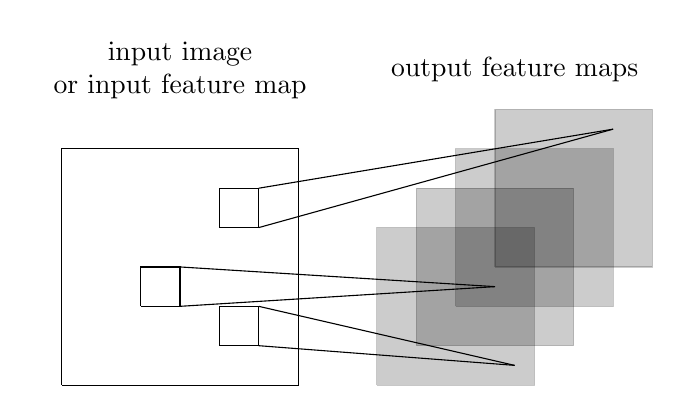
\begin{tikzpicture}
		\node at (1.5,4){\begin{tabular}{c}input image\\or input feature map\end{tabular}};
	
		\draw (0,0) -- (3,0) -- (3,3) -- (0,3) -- (0,0);
		
		\draw (2,2) -- (2.5,2) -- (2.5,2.5) -- (2,2.5) -- (2,2);
		\draw (2,0.5) -- (2.5,0.5) -- (2.5,1) -- (2,1) -- (2,0.5);
		\draw (1,1) -- (1.5,1) -- (1.5,1.5) -- (1,1.5) -- (1,1);
		
		\draw (2.5,2) -- (7,3.25);
		\draw (2.5,2.5) -- (7,3.25);
 
		\draw (2.5,1) -- (5.75,0.25);
		\draw (2.5,0.5) -- (5.75,0.25);
		
		\draw (1.5,1.5) -- (5.5,1.25);
		\draw (1.5,1) -- (5.5,1.25);
		
		\node at (5.75,4){\begin{tabular}{c}output feature maps\end{tabular}};
		
		\draw[fill=black,opacity=0.2,draw=black] (5.5,1.5) -- (7.5,1.5) -- (7.5,3.5) -- (5.5,3.5) -- (5.5,1.5);
		\draw[fill=black,opacity=0.2,draw=black] (5,1) -- (7,1) -- (7,3) -- (5,3) -- (5,1);
		\draw[fill=black,opacity=0.2,draw=black] (4.5,0.5) -- (6.5,0.5) -- (6.5,2.5) -- (4.5,2.5) -- (4.5,0.5);
		\draw[fill=black,opacity=0.2,draw=black] (4,0) -- (6,0) -- (6,2) -- (4,2) -- (4,0);
	\end{tikzpicture}
	\caption{Illustration of a convolutional layer.}
	\label{fig:convolutional-layer}
\end{figure} When stemming from numerous sources, large datasets can exponentially increase the number of nodes in convolution. Large datasets are likely to benefit from recurrence (RNN). 

RNN models are designed for temporal or sequentially indexed data, effectively managing time dependencies. They maintain hidden states, which allow for the integration of past information across an ordered sequence, as opposed to the moving window approach utilized by CNNs. Combining Convolutional Neural Networks (CNN) and Recurrent Neural Networks (RNN) results in Hierarchical Convolutional Recurrent Neural Networks (HCRNN), thereby enhancing classification accuracy in multi-spectral, time-varying geospatial datasets. The general MLP is depicted in figure \ref{fig:multilayer-perceptron} where $D$ input units and $C$ output units will be tested in this thesis. \begin{figure}[t]
	\centering
	\begin{tikzpicture}[shorten >=1pt]
		\tikzstyle{unit}=[draw,shape=circle,minimum size=1.15cm]
		%\tikzstyle{hidden}=[draw,shape=circle,fill=black!25,minimum size=1.15cm]
		\tikzstyle{hidden}=[draw,shape=circle,minimum size=1.15cm]
 
		\node[unit](x0) at (0,3.5){$x_0$};
		\node[unit](x1) at (0,2){$x_1$};
		\node at (0,1){\vdots};
		\node[unit](xd) at (0,0){$x_D$};
 
		\node[hidden](h10) at (3,4){$y_0^{(1)}$};
		\node[hidden](h11) at (3,2.5){$y_1^{(1)}$};
		\node at (3,1.5){\vdots};
		\node[hidden](h1m) at (3,-0.5){$y_{m^{(1)}}^{(1)}$};
 
		\node(h22) at (5,0){};
		\node(h21) at (5,2){};
		\node(h20) at (5,4){};
		
		\node(d3) at (6,0){$\ldots$};
		\node(d2) at (6,2){$\ldots$};
		\node(d1) at (6,4){$\ldots$};
 
		\node(hL12) at (7,0){};
		\node(hL11) at (7,2){};
		\node(hL10) at (7,4){};
		
		\node[hidden](hL0) at (9,4){$y_0^{(L)}$};
		\node[hidden](hL1) at (9,2.5){$y_1^{(L)}$};
		\node at (9,1.5){\vdots};
		\node[hidden](hLm) at (9,-0.5){$y_{m^{(L)}}^{(L)}$};
 
		\node[unit](y1) at (12,3.5){$y_1^{(L+1)}$};
		\node[unit](y2) at (12,2){$y_2^{(L+1)}$};
		\node at (12,1){\vdots};	
		\node[unit](yc) at (12,0){$y_C^{(L+1)}$};
 
		\draw[->] (x0) -- (h11);
		\draw[->] (x0) -- (h1m);
 
		\draw[->] (x1) -- (h11);
		\draw[->] (x1) -- (h1m);
 
		\draw[->] (xd) -- (h11);
		\draw[->] (xd) -- (h1m);
 
		\draw[->] (hL0) -- (y1);
		\draw[->] (hL0) -- (yc);
		\draw[->] (hL0) -- (y2);
 
		\draw[->] (hL1) -- (y1);
		\draw[->] (hL1) -- (yc);
		\draw[->] (hL1) -- (y2);
 
		\draw[->] (hLm) -- (y1);
		\draw[->] (hLm) -- (y2);
		\draw[->] (hLm) -- (yc);
 
		\draw[->,path fading=east] (h10) -- (h21);
		\draw[->,path fading=east] (h10) -- (h22);
		
		\draw[->,path fading=east] (h11) -- (h21);
		\draw[->,path fading=east] (h11) -- (h22);
		
		\draw[->,path fading=east] (h1m) -- (h21);
		\draw[->,path fading=east] (h1m) -- (h22);
		
		\draw[->,path fading=west] (hL10) -- (hL1);
		\draw[->,path fading=west] (hL11) -- (hL1);
		\draw[->,path fading=west] (hL12) -- (hL1);
		
		\draw[->,path fading=west] (hL10) -- (hLm);
		\draw[->,path fading=west] (hL11) -- (hLm);
		\draw[->,path fading=west] (hL12) -- (hLm);
		
		\draw [decorate,decoration={brace,amplitude=10pt},xshift=-4pt,yshift=0pt] (-0.5,4) -- (0.75,4) node [black,midway,yshift=+0.6cm]{input layer};
		\draw [decorate,decoration={brace,amplitude=10pt},xshift=-4pt,yshift=0pt] (2.5,4.5) -- (3.75,4.5) node [black,midway,yshift=+0.6cm]{$1^{\text{st}}$ hidden layer};
		\draw [decorate,decoration={brace,amplitude=10pt},xshift=-4pt,yshift=0pt] (8.5,4.5) -- (9.75,4.5) node [black,midway,yshift=+0.6cm]{$L^{\text{th}}$ hidden layer};
		\draw [decorate,decoration={brace,amplitude=10pt},xshift=-4pt,yshift=0pt] (11.5,4) -- (12.75,4) node [black,midway,yshift=+0.6cm]{output layer};
	\end{tikzpicture}
	\caption[Network graph for a $(L+1)$-layer perceptron.]{Network graph of a $(L+1)$-layer perceptron with $D$ input units and $C$ output units. The $l^{\text{th}}$ hidden layer contains $m^{(l)}$ hidden units.}
	\label{fig:multilayer-perceptron}
\end{figure} These offer powerful future directions for this thesis and the means to address numerous gaps in surface O$_3$ literature; an MLPR combined with a spatial temporal regression of uncertainty can be thought of as a basic implementation of an HCRNN with the use of geospatial kernels as their sequencing strategy. HCRNNs have shown great promise for depicting surface O$_3$ data sets and modeling air pollution trends, but still produce high geospatial error in dense urban locations (\cite{mandal_bivariate_2024}; \cite{kleinert_intellio3-ts_2020}; \cite{sun_improvement_2021}) due to the lack of spatial associations. 
%%%%%%%%%%%%%%%%%%%%%%%%%%%%%%%%%%%%%%%%%%%%%%%%%%%%%%%%%%%%%%%%%%%%%%%%%%%%%%%%%%%%%%%%%%%%%%%%%%%%%%%%%%%%%%%%%%%%
\section{Gaps in Surface O$_3$ Literature} \label{litreview:gaps} As has been the case with all the ensembles mentioned, geospatial uncertainty has not yet been fully integrated. Another obvious gaps in the literature is the complete coverage of rasterized data depicting surface O$_3$ values for the United States. As is with most cases regarding high-resolution data, many specialized forms of surface O$_3$ exist, but have yet to be incorporated into high-resolution raster models depicting universal surface trends, save a few case studies such as this thesis (e.g., \cite{choi_summertime_2012}; \cite{rui_zhu_rapid_2023}; \cite{xiao_lu_wildfire_2016}). Many high resolution models have been created for the EU, China, India, Iran, and other urbanized nations similarly concerned with the growing rate of surface O$_3$ reactions (\cite{dong_assessment_2021}; \cite{li_estimation_2023}; \cite{tian_assessing_2024}). Urban based public health case studies tend to focus on personal exposures from environmental aspects related to O$_3$. These studies typically assign O$_3$ concentrations to willing participants through advanced statistical models, using geo-located addresses to predict individual exposure to surface O$_3$ (\cite{ghozikali_effect_2015}; \cite{jerrett2009}; \cite{crouse_ambient_2015}; \cite{turner_long-term_2016}). 

The information provided by exposure studies tends to be highly informative for modeling due to their nature as high-resolution datasets. These studies are typically based on satellite measurements, such as normalized differential vegetation index (NDVI) and temperature estimates. However, they do not provide a complete depiction of the area, as their focus is on exposure analysis rather than transport mechanics. Most exposure models are difficult to create, as the movement of a human can drastically change exposures to other harmful pollutants, let alone surface O$_3$ which potentially co-funds with NO$_x$ and PM$_2.5$ constituents \cite{malley_updated_2017}; \cite{vardoulakis_intra-urban_2011}; \cite{turner_long-term_2016}). Interactions with these constituents, along with other volatile organic compounds (VOCs) and naturally occurring chemicals in Earth’s atmosphere, as explained in Chapter \ref{introchap:twolayers}, suggest that anthropogenic sources and isoprene-related VOCs tend to exhibit the strongest correlations with surface O$_3$ reactions (\cite{wang_evolution_2023}; \cite{nelson_comprehensive_2023}; \cite{ni_surface_2024}). 

When exposed over long-terms, O$_3$ has potential associations with hospitalization rates of upper and lower respiratory diseases. These associations vary with age, gender, and the individual's initial health. Additionally, O$_3$ promotes unnecessary and unregulated oxidative stress, leading to irreversible cognitive and immune system damage (\cite{barzeghar_long-term_2020}; \cite{fania_machine_2024}; \cite{luan_assessment_2024}). Numerous studies worldwide have identified minor to major associations between short-term exposure at the surface during seasonal cycles, which have potential direct and indirect consequences that are still under discussion (\cite{marx_short_2020}; \cite{ma_short-term_2023}; \cite{zhang_short-term_2023}). The observed trend is understandable due to the chemical volatility of O$_3$, as oxidative stress becomes easier to achieve with O$^{-}$, a product of unstable O$_3$, rather than solely O$_2$ \cite{cai_oxidative_2022}. Within O$_3$ models for health-related risk, policy making, or similar cohort-based studies; air pollution, along with growing worries of climate change, and associated health risks, has spurred the need for high-resolution imagery at around 300 m (\cite{wang_does_2023}). 

The most notable gap in O$_3$ literature is the same found with all ML/AI representations of geospatial data. Due to the revolution in Big Data and scientific technology, in situ surface measurements are readily available throughout the world (\cite{gaudel_tropospheric_2018}; \cite{schultz_tropospheric_2017}). Researchers specializing in hybrid ML/AI methods for geospatial data typically do not incorporate these in situ measurements in the final prediction. Simply using them during the training process can establish an accurate trend based on corrections made by remote sensing satellites; however, these satellites do not rely on ground-based observations. Chapter III later mentions that all remote sensing images are based on corrected measurements of reflected light. When applied to coarse resolutions, these errors can be negligible due to the large area they’re meant to describe (about 1 km and above). Remote sensing data utilized for these also only represent total column estimates, not complex surface interactions. while accurate, at a high resolutions from ~500 m to 1 km, and covering national boundaries, they still depict some error regarding tropospheric chemicals in the upper and lower hemispheres of Earth when using remotely sensed imagery at resolutions below 500 m.
%%%%%%%%%%%%%%%%%%%%%%%%%%%%%%%%%%%%%%%%%%%%%%%%%%%%%%%%%%%%%%%%%%%%%%%%%%%%%%%%%%%%%%%%%%%%%%%%%%%%%%%%%%%%%%%%%%%%
\section{Conclusion} \label{litreview:litconc} Models covered in this chapter helped better understand the complex processes governing O$_3$ formation and transport. These are ultimately used by decision makers on all scales and influence decisions surrounding efforts to mitigate the impacts of constituents attributing to surface O$_3$ prominence (\cite{du_policy_2024}; \cite{balamurugan_tropospheric_2021}; \cite{wang_policy-driven_2021}). Given this information, it was expected that the data set would need to be as complex as the reaction itself, requiring many features to accurately represent known interactions O$_3$ has with natural and built environments (\cite{gao_large-scale_2023}; \cite{sanchez_evaluation_2008}; \cite{wang_urbanization_2024}). Studies with a brief depiction, section, or which focus on surface O$_3$ entirely suggest the best models suited for this project are tree-based and neural network models.  

Many tropospheric O$_3$ transport models assume constant distribution of the gas over the system in question and only result in predictions at a resolution of around 4 km. CTM models are employed in a wide variety of studies due to the robustness of their methodology; the computational expenses arise from the significant effort required to optimize the model, depending on the complexity of the gas in question. For O$_3$, these models are often complex but imperative to ensure a safe future for current and future generations. The health impacts and concerns associated with surface O$_3$ exposure can’t rely CTM based models due to the coarse results , which tend to underestimate or overestimate O$_3$ concentrations in the upper and lower and upper latitudes, respectively (\cite{solomou_evaluating_2018}; \cite{yu_errors_2018}).

Researchers have developed interpolated exposure rates via temporal analysis of extrapolated statistical learning models to create unique activity space exposures (\cite{malley_updated_2017}; \cite{turner_long-term_2016}; \cite{crouse_ambient_2015}). These are extremely fine resolution; however, depicting exposures in-terms of the populations exposed space. As the models in this thesis are trained on data gathered from similar exposure analyses and satellite observations, developing a large dataset that combines these techniques may improve exposure assignment times by reducing the coding work necessary to incorporate O$_3$ as a variable of interest. This work could benefit numerous case studies in areas related to, but not limited to, public health, surface chemistry and air quality, environmental health, atmospheric health, chemical transport trends, and other similar methodologies. The culmination of this research is used for the Statistical Modeling and Residual Kriging (SMaRK) methodology which implements numerous feature transformations and spatial-temporal analytics to test unique data sets across the AOI.